\chapter{Music}
\label{Music}
\section{Navigating Sonically}
\label{sonicnav}
I have developed a theoretical system for using sound to navigate a
higher-dimensional space, using ideas from \emph{Harry Partch} and \emph{Joe
Monzo's} approached to tuning theory.

This is a process to generate intervals based on a set of spatial coordinates,
or simply a set of parameters. Taking inspiration from the
\emph{just-intonation} tuning method a ratio comprised of integers only sounds
consonant.

Tuning theory is a fundamental question when it comes to developing musical
systems, the common myth as told by Iamblichus is that Pythagoras was ``walking
near a brazier's shop, he heard from a certain divine casualty the hammers
beating out a piece of iron on an anvil, and producing sounds that accorded with
each other.'' \citep[p.62]{iamblichus} Pythagoras had discovered that hammers of
certain weights were consonant with each other musically. This leads to the
concept of intervals.

\subsection{Intervals}
An \emph{interval} is simply a ratio of two frequencies: $\frac{f_1}{f_2}$.
Pythagoras' hammers were consonant as their weights were 12, 9, 8, and 6.  The
ratios here of $12:6$ correspond to $\frac{2}{1}$ or an octave, similarly $12:9
= \frac{4}{3}, 12:8 = \frac{3}{2}$ for the other two. Whilst this myth is
probably apocryphal, the use of ratios of strings for music has been used since
antiquity. What Pythagoras proved is that intervals are these ratios and that
materials have properties from which these frequencies arise.

\begin{figure}[H]
    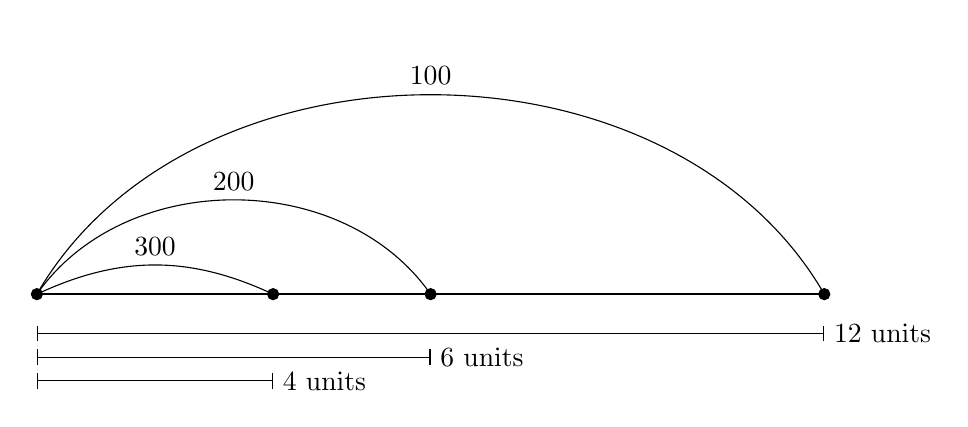
\begin{tikzpicture}
        %'string'
        \draw[-, thick] (-5, 0) -- (5, 0);
        \node at (-5, 0) {\pgfuseplotmark{*}};
        \node at (5, 0) {\pgfuseplotmark{*}};
        \node at (0, 0) {\pgfuseplotmark{*}};
        \node at (-2, 0) {\pgfuseplotmark{*}};
        
        % frequencies
        \draw[-, bend left=60] (-5, 0) to node[above] {$100\si{\hertz}$} (5, 0);
        \draw[-, bend left=55] (-5, 0) to node[above] {$200\si{\hertz}$} (0, 0);
        \draw[-, bend left=25] (-5, 0) to node[above] {$300\si{\hertz}$} (-2, 0);

        % lengths
        \draw[-, arrows=|-|] (-5, -0.5) -- (5, -0.5) node[right] {$12$ units};
        \draw[-, arrows=|-|] (-5, -0.8) -- (0, -0.8) node[right] {$6$ units};
        \draw[-, arrows=|-|] (-5, -1.1) -- (-2, -1.1) node[right] {$4$ units};
    \end{tikzpicture}
    \centering
    \caption{Diagram showing intervals being related to the idea of a ratio of
    lengths for example the $300\si{\hertz}$ frequency is related to the
    $200\si{\hertz}$ frequency by $\frac{6}{4} = \frac{3}{2}$}
\end{figure}

Pythagoras then set about creating a tuning system based around the
$\frac{3}{2}$ ratio (the perfect fifth). The perfect fifth is the most consonant
ratio that is not unison or an octave \footnote{It is named so because of
musical convention, it being five notes between notes in a scale, it has no
direct relation to the ratio of $1.5$}. Using this ratio we can combine the
numbers $2$ and $3$ to different powers to generate intervals. For example $2^0
3^0 = 1$ or unity, other intervals can be generated but we run into a problem.
Using this method of moving in $\frac{3}{2}$ increments if we try to go 7
octaves i.e.  $(\frac{2}{1})^7 = 128$ vs 12 fifths \footnote{These should be the
same see: the circle of fifths} we get $(\frac{3}{2})^{12} =
129.7463379\ldots$ the ratio of these two different values is
$\frac{(1.5)^{12}}{2^7} \approx 1.01364$. In essence the comma's existence can
be surmised by: there exists no $n \neq 0$ such that $2^n = 3^n$. This is
important as it marks the difference from the system we use in the west today
called `12-tone equal temperament' which divides an octave into 12 equal tones
of $2^{\frac{1}{12}}$ to solve this problem.

For our purposes we will be using intervals, ratios of frequencies, to generate
new frequencies or notes for use in the program. If we generate a ratio then we
may simply multiply a frequency to find the frequency of the other note $x \cdot
\frac{f_1}{f_2} = y$.

A \emph{$p$-limit} tuning system is a just-intonation based system where every
interval's highest prime factor is $p$. \citep[p.76, 109]{partch1974genesis}
Pythagoras' tuning system can be said to be 3-limit. These intervals can be
represented using an exponent vector, usually called a `monzo'
\citep{monzo_2005}; for example, $3:2$ is represented as such: $|-1\ 1\ \rangle$.
This is simply a shorthand for $2^{-1} 3^1$, and can be extended: $|e_1\ e_2\
\cdots\ e_n\rangle$ where each $e_i$ in the vector is an exponent of a prime
number $2^{e_1} 3^{e_2} \cdots p_n^{e_n}$. 

Often these vectors are shown as $|*\ e_2\ \cdots\ e_n \rangle$ The $*$ represents the idea
of octave equivalence, a musical idea that a doubling of the frequency produces
a note that is `the same', and as such any value of exponent for the $2$ can be
placed there. As an example $|1\ 1\rangle = 2^0 3^1 = \frac{3}{1}$ but this is
equivalent to $\frac{3}{2}$, as you can simply halve the frequency produced by
the ratio to get back to it. To normalise the interval the same octave, set the
constraints $1 \leq \frac{f_1}{f_2} < 2$ and similarly for other octaves higher
or lower, just halving and doubling the bounds.

\subsection{Navigating Space}
\subsubsection{In 2D}
Assume a base frequency, $440\si{\hertz} = f_1$. As an example, if the user was
at $x=1$, $y=-1$.

\begin{figure}[H]
    \centering
    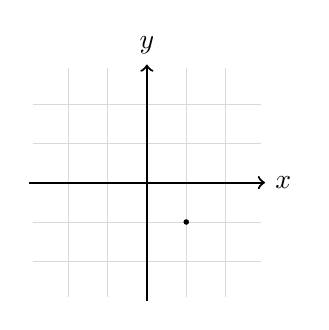
\begin{tikzpicture}[scale=0.5]
        \draw[help lines, color=gray!30](-2.9, -2.9) grid (2.9, 2.9);
        \draw[->, thick] (-3,0) -- (3,0) node[right]{$x$};
        \draw[->, thick] (0,-3)-- (0,3) node[above]{$y$};

        \fill (1,-1) circle[radius=2pt];
    \end{tikzpicture}
    \caption{}
\end{figure}

This is represented in the vector $|0\, 1\, -1\rangle$ which corresponds to $2^0
3^1 5^{-1} = \frac{6}{5}$. $\frac{6}{5}$ is a minor-third, and represents
$528\si{\hertz}$, this is consonant.

Or in general:
\begin{align*}
    2^n \cdot 3^x \cdot 5^y \cdot f_1 &= f_2
\end{align*}

If the user is at non-integer numbers for $x$ and $y$ we can calculate the frequencies too.
\begin{figure}[H]
    \centering
    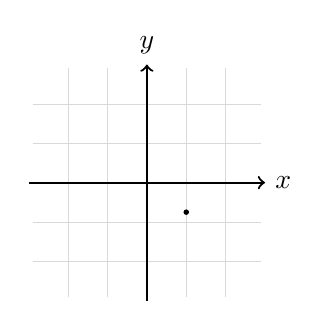
\begin{tikzpicture}[scale=0.5]
        \draw[help lines, color=gray!30](-2.9, -2.9) grid (2.9, 2.9);
        \draw[->, thick] (-3,0) -- (3,0) node[right]{$x$};
        \draw[->, thick] (0,-3)-- (0,3) node[above]{$y$};

        \fill (1,-0.75) circle[radius=2pt];
    \end{tikzpicture}
    \caption{}
    \label{outoftune}
\end{figure}

Where $x=1$ and $y=-0.75$ we can simply find the frequency as $2^0 \cdot 3^1
\cdot 5^{-0.75} \cdot 440\si{\hertz} = 394.772\si{\hertz}$. This will sound
dissonant and not particularly nice.

The idea here is simple, generating intervals like this allows for some points
in space to be consonant and others to be dissonant, these could correspond
visually with some output being produced by the program but should hopefully
allow a user to differentiate between points in space using their sense of
hearing.

\subsubsection{In Higher Dimensions}
This idea extends into higher dimensions naturally, simply adding to the number
of terms in the vector $|*\ e_3\ e_5\ \cdots\, e_p\  \rangle$. Each of these
exponents could represent some parameter added to the program. 

\subsection{Limitations}
As more variables are introduced integer ratios will sound less `strongly
consonant' and may be harder to understand naturally. However, every interval
that is possible with fewer variables will still be possible so a user could
still explore one or two parameters at a time and get the same results.

\subsection{Processing Demo}
I have created a demo of this concept in 2D in processing, the code is in
\autoref{audiodemo}. The program simply has an integer-marked grid that the user
can navigate using \verb|WASD| and will calculate the interval based on the
coordinates of the point. Similarly to \autoref{outoftune}:

\begin{figure}[H]
\centering
\subfloat{\tikz[remember
picture]{\node(1AL){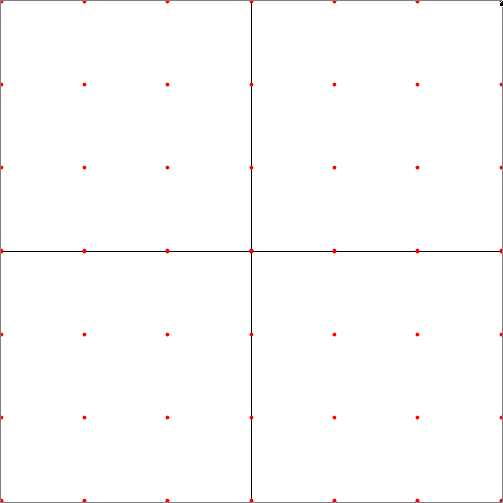
\includegraphics[width=.4\textwidth]{audiopoc2}};}}%
\hspace*{2cm}%
\subfloat{\tikz[remember
picture]{\node(1AR){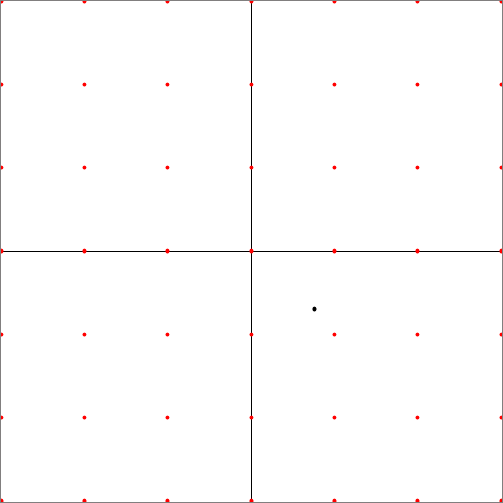
\includegraphics[width=.4\textwidth]{audiopoc1}};}}
\caption{At first the black dot is hidden beneath the centre red dot, the user uses WASD to navigate,
the audio is out of tune in the second state}
\end{figure}
\tikz[overlay,remember picture]{\draw[-latex,thick] (1AL) -- (1AL-|1AR.west)
node[midway,below]{};} 

This demo is simple and only uses two sine waves so is unpleasant to listen to,
but illustrates the point, at points outside those marked there is a `beating'
sound to the waves as they do not harmonise correctly. However, as some points
aren't marked that \emph{do} sound somewhat consonant, so this cannot be the
only navigation method , only a prompt to help the user.
\section{Composition}
\label{Composition}
To create a sound accompaniment to the visual aspect we first need to consider
what style of music we should explore, that is to say, create at least an idea
of composition. Generative music is the technique we're exploring here, with
musical ideas being emergent from a set of parameters, and created from a system
that processes them. The definition is vague as with generative art, the main
requirement is that a system is set up and creates the music, this doesn't need
to be a computer, but often is.

Generative music is rather recent, with Brian Eno being major figure
popularising its use, he would often use the analogy of a Moir\'{e} pattern to
describe how the programs would work at the time.  

The immediate style of music to draw from Viner's work would probably be that of
minimalism, the repetition and difference across an image is similar in style to
especially the percussive works of Reich, Glass, Riley, and even the drone works
of La Monte Young to an extent. Another, less famous example that I feel conveys
the feeling well is \emph{Jon Gibson - Cycles (1977)}, the cover for the
recording is a Moir\'{e} pattern, and the work modulates a 7-note pattern that
comes into and out of phase with itself.

Eno refers to his inspiration of generative music to be triggered by
hearing \emph{It's Gonna Rain} by Reich, linking generative music as a concept
pretty solidly to Minimalism. Reich used the analogy of fabric work and weaving,
featuring on the cover of Music for 18 Musicians is a woven piece of fabric;
this seems similar to the idea of a grid (given that weaving takes place on a
matrix of strings, perhaps the crossing points could be seen as `vertices')

Overall the idea with the composition should be to enhance what is on the
screen if the image is disordered the sound should be too, if it is ordered
and regular the sound should follow. If there are some number of vertices in the
shapes on the screen there should be some feedback too.

Further, this will be combined with the methods mentioned in
\autoref{sonicnav}, including the ideas present in the mentioned minimalist
composers. This will be an element in the work that is unique from the art and
perhaps helps distance itself from being purely a replica of Viner.

\section{Synthesis}
Broadly there are four approaches to digital synthesis, that of: the processed
recording; the spectral model; the physical model; and the abstract algorithm
\citep{smith_2005}.

For this project, spectral and physical modelling is out of the scope and would
require more specialist audio software frameworks. Processed recording, includes
more sample-based audio and manipulation of that, granular synthesis is an
example. The 'abstract algorithm' methods include things like FM synthesis,
which in its most basic form is comprised of a carrier waveform whose frequency
is modulated by another waveform, this can be extended by things like including
feedback at various stages of the processing.

On top of these methods, there should also be a consideration to audio effects,
processing and p5.js both have sound libraries with built-in audio effects,
reverb and delay perhaps being the most important to create the idea of a space
in the sound.

Creating these methods in software is straightforward when there is already
some digital signal processing in place; a library called \verb|Tone.JS| handles
the practicalities of generating sound in JavaScript and works alongside
\verb|p5.js| nicely.

Additive synthesis makes sense for use here there are a lot of controls over
parameters, it is easy to implement and can reproduce many different qualities
of sound.  As in the composition section, work like `Cycles' is performed on the
organ for example. This is an easy sound to replicate in additive synthesis as
you can achieve the effect by playing multiple sine waves at the same time; this
is what the earliest pipe-less organs did. Whilst not in software, they would
have series of plates or disks that encoded the waveforms and played them all at
once through a mixer to create complex waveforms \citep{10.2307/3680869}.

\subsection{Additive Synthesis in Tone.JS}
First I have created a bank of oscillators that can be tuned to any frequency
and triggered. I can loop through these and use an `envelope' consisting of to
control the volume over time of all of them at once, this is simply set as such:

\begin{lstlisting}[language=JavaScript]
const env = new Tone.AmplitudeEnvelope({
    attack:1,
    decay: 2,
    sustain: 1,
    release: 0.3
});
\end{lstlisting}

\begin{figure}[H]
    \centering
    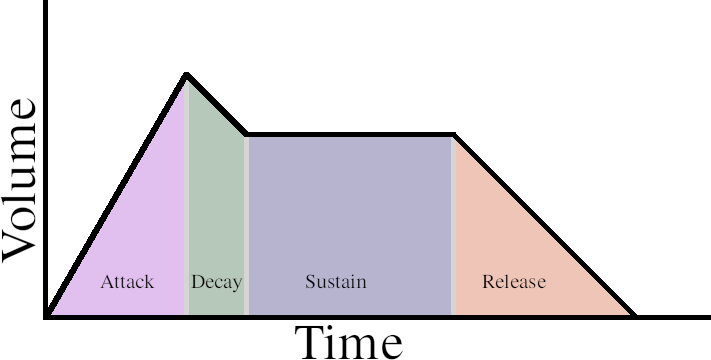
\includegraphics[width=0.6\textwidth]{adsr}
    \caption{Typical attack decay sustain release (ADSR) curve}
\end{figure}

The number of oscillators in a bank can be chosen at will and for our purposes
are tuned as per the harmonic series this is to create a pleasing timbre (the
`summation' or additive part is when we feed them into a mixer). 
Each oscillator is labelled with a number that corresponds to the term of the
harmonic series, when the attack for each oscillator is triggered the frequency
is calculated as the incoming frequency times the number of the term. Also, each
oscillator will be quieter than the last according, this is again to create
the timbre.

Since we are adding these oscillators' signals together, consideration needs to
be given to the phase angle that each lay at. Setting them to \verb|(i / NUM_OSCS) * 360| 
will allow for there to be no harsh constructive or destructive interference
between the oscillators.


\section{Sequencing}
\label{Sequencing}
To create a sequence I considered a couple of options, to have a fixed note
sequence for example. This would perhaps be too static and not fit with the idea
of the project being generative art. Another simple option was to make notes
completely random, this tends to sound `robotic' like a Sci-Fi movie control
panel. There could also be a random choice within a set of consonant notes (i.e.
that of a chord) this is a better idea because there's less chance of a `bum
note' (one that sounds out of place).

An extension of this idea is to use Markov Chains to model music in
\citep{ballstate2016} for example, they analyse Bach, Mozart, Palestrina, and
Beethoven to create a set of transition matrices for their chord progressions.
In this example, chord progressions are used but the method can easily be adapted
to note progressions too. 

For my sequence, I picked six possible tones, expressed as intervals from a base
tone, as $1, 1.2, 1.25, 1.5, 1.6, 2$ these represent unison, a minor third, a
major third, perfect fifth, and a minor sixth, and the octave (all
just-intonation). These tones were picked because they were the intervals in
5-limit that didn't have recurring decimals.\footnote{Ultimately this is arbitrary but
ends up fitting the definition of an augmented scale, this type of scale was
used more extensively in the 20th Century in Jazz, it was also used in Listz's
`Faust's Symphony'. Another way of thinking about it is two major triads above a
base pitch (e.g. C E G and E Eb Ab).} Each tone is also then affected by the
interval generated above to create a possible series of tones that depend on the
parameters of the program.

To create a Markov chain sequence first a matrix of probabilities that represent
the chain needs to be created. This defines the possible transitions between
notes and the probabilities of them, each row should add to give a total
probability of $1$. Changing the values in this matrix can therefore be thought
of as composing what series of tunes are possible and probable.

\[
\begin{blockarray}{ccccccc}
    & 1 & 1.2 & 1.25 & 1.5 & 1.6 & 2\\
    \begin{block}{c (cccccc)}
        1    & 0  & 0.2& 0.5& 0.1& 0.1& 0.1\\
        1.2  & 0.1& 0  & 0.4& 0.1& 0.2& 0.2\\
        1.25 & 0.3& 0  & 0.1& 0.4& 0.1& 0.1\\
        1.5  & 0.3& 0.2& 0.2& 0  & 0.1& 0.2\\
        1.6  & 0.2& 0.2& 0.2& 0.3& 0  & 0.1\\
        2    & 0.4& 0.1& 0.2& 0.2& 0.1& 0  \\
    \end{block}
\end{blockarray}
\]

This represented in code becomes: 
\begin{lstlisting}[language=Javascript]
const markovObject = {
                        1:    [0  , 0.2, 0.5, 0.1, 0.1, 0.1],
                        1.2:  [0.1, 0  , 0.4, 0.1, 0.2, 0.2],
                        1.25: [0.3, 0  , 0.1, 0.4, 0.1, 0.1],
                        1.5:  [0.3, 0.2, 0.2, 0  , 0.1, 0.2],
                        1.6:  [0.2, 0.2, 0.2, 0.3, 0  , 0.1],
                        2:    [0.4, 0.1, 0.2, 0.2, 0.1, 0  ]
                    };
\end{lstlisting}

Using an object allows for fast lookup, then each index in the object refers to
an index of the keys of the object. So picking the next is simple, generate a
random number from 0 to 1 and then accumulate probability until we reach it:

\begin{lstlisting}[language=Javascript]
probList.forEach((e, i) => {
    if (picked >= acc && picked < acc + e) {
        intervalIndex = i;
    }
    acc += e;
});
\end{lstlisting}

Where \verb|probList| is the array referenced by the key of the current note in the
object and \verb|intervalIndex| is the index of the array of keys in the object.

Overall this is a simple method for creating note sequences but is effective for
limiting the number of possible transitions with a lot of flexibility.  

\section{Chords}
For the music to not sound one-dimensional we need to pick more than one note to
play in the additive synthesis. This leads to the idea of chords, again we can
build these with intervals, this time using a bit more music theory. 

I chose that for each vertex that is present in the middle of the screen there
should be another note in the chord. The structure of the chord I chose is
simple with the notes being the base note, the minor third, the fifth, the minor
seventh, the octave, and the whole tone (or 2nd). Represented by the ratios $1,
\frac{6}{5}, \frac{3}{2}, \frac{9}{5}, 2, \frac{9}{8}$ respectively. This is
purely an artistic choice. For example, if a triangle is in the centre of the
screen the first three intervals in the chord will be played $1, \frac{6}{5},
\frac{3}{2}$ resulting in a minor fifth chord. If the user then moves on top of
a square the $\frac{9}{5}$ ratio is added to the chord making a minor seventh,
similarly, if there's a pentagon it simply adds an octave and for a hexagon, a
whole tone which will sound strange but hexagons are rarer to find, making it
feel `special'.

To implement this I simply store the chord in a function expression that returns
the frequency to set each voice (oscillator bank) to in an array up to the index
\verb|i|. Then another function expression that triggers the release on voice
and attack with the new frequency.

\begin{lstlisting}[language=JavaScript]
const getChord = (i) => [
    base*currentNote,
    base*currentNote*1.2,
    base*currentNote*1.5,
    base*currentNote*1.8,
    base*currentNote*2,
    base*currentNote*1.125
];

const playVoice = (note, time) => {
    voiceIndex++;
    voiceIndex = voiceIndex % bvoices.length;
    bvoices[voiceIndex].triggerRelease(time);
    mvoices[voiceIndex].triggerRelease(time);
    bvoices[voiceIndex].triggerAttack(note, time);
    mvoices[voiceIndex].triggerAttack(note*interval, time);
};
\end{lstlisting}

Since the number of possible notes to play at once is 6, the voices array
contains six oscillator banks, each with 4 oscillators in them leading to 24
sine waves oscillators at once at maximum. There are two arrays of voices for
the base and movable voice so overall there are 48 sine oscillators.

Extensions of this method may lend themselves to being able to control the
waveform types and phase of each of the waves as well as what harmonics are
present in each voice. Also the ability to change the intervals in a chord.
These seem less important for an application such as this primarily static
artistic use.
